\section{Integration into Visualization Tools}

Throughout the life of the ECP, the \vtkm team collaborated heavily with other ECP software technology teams.
The scope of the \vtkm project was to provide the fundamental technology to run scientific visualization algorithms on GPUs, which account for the vast majority of the computational power of current exascale machines.
Other ECP teams, most notably the ALPINE project, developed tools that would leverage \vtkm while directly addressing application needs.
This arrangement avoided the redundant work of multiple teams developing their own visualization solutions and prevented users from having to use yet another software interface.
In this section, we discuss the major visualization tools that we integrated \vtkm with.

%% \ken{
%%   Each subsection should be roughly 1/2 page plus have an image demonstrating the tool with \vtkm that is about 1/3 page.
%%   (3 + 1/3 page total.)
%%   The subsection should start with a description of the tool.
%%   (Exception: the last subsection starts with a description of the lengthy process from committing code in \vtkm to it being available in a tool.)
%%   The following paragraphs describe how \vtkm is integrated at a high level.
%%   Avoid details like classnames.
%% }

\subsection{ParaView}

%\assign{Sujin}
The \vtkm library provides high-performance implementations of several visualization algorithms for highly parallel processors.
However, features such as file I/O, rendering, and pipeline management, which are all essential parts of a full-featured visualization toolkit, are beyond the scope of \vtkm.
On the other hand, ParaView is a mature visualization software that has robust implementations of these features.
Therefore, we wanted to integrate \vtkm into ParaView in such a way that ParaView can use \vtkm filters to accelerate its operations when a \vtkm implementation and highly parallel hardware is available.

We also wanted the \vtkm accelerated filters to be as easy to use as possible.
Therefore, we chose to integrate \vtkm using VTK and ParaView's factory-instantiation feature.
Because ParaView is implemented on top of VTK and internally relies on VTK filters, both VTK and ParaView will be mentioned interchangeably in this section.
Filters in ParaView are instantiated via a factory method.
There can be multiple implementations available for a filter, and the factory method chooses an appropriate implementation at run time based on given criteria.
With this method, we can override the default ParaView filters with \vtkm-based filters.
Currently, \vtkm accelerated filters that override traditional CPU implementations are available for some commonly used filters such as contour, threshold, and gradient.
%Adding overrides for more filters is a straightforward process as discussed in the following paragraphs.
Additional \vtkm filters can be added by providing additional overrides.

To override a ParaView filter, we first need to implement a \vtkm wrapper filter in VTK to provide the interface of the base VTK/ParaView filter and use \vtkm filters and routines for its operation. The following steps provide a high-level overview of how a \vtkm wrapper filter is implemented in VTK/ParaView:
\begin{enumerate}
    \item Check the filter parameters and only proceed with \vtkm processing for configurations supported by the \vtkm filter implementation.
    \item Convert the input VTK datasets to \vtkm datasets. 
    \item Execute the \vtkm filter on the data.
    \item Convert the output of the \vtkm filter back to VTK datasets.
    \item If an error occurs at any point during the above steps, then fall back to the default VTK implementation. Errors in \vtkm are typically signaled via C++ exceptions.
\end{enumerate}

For the dataset conversion from VTK to \vtkm and back, we implemented several helper routines. These are zero-copy operations for most cases because, whenever possible, only the ownership of the pointers to the underlying resources is transferred. Even copies from host-to-device and device-to-host are minimized by using a \vtkm dataset wrapper in VTK called \texttt{vtkmDataSet}, which implements the \texttt{vtkDataSet} interface and only copies the data when required. Another commonly used ParaView functionality is computing the range of the various fields of a dataset. This has also been accelerated by using \vtkm, which speeds up the computation and avoids memory transfer from device to host.

\begin{figure}[t]
  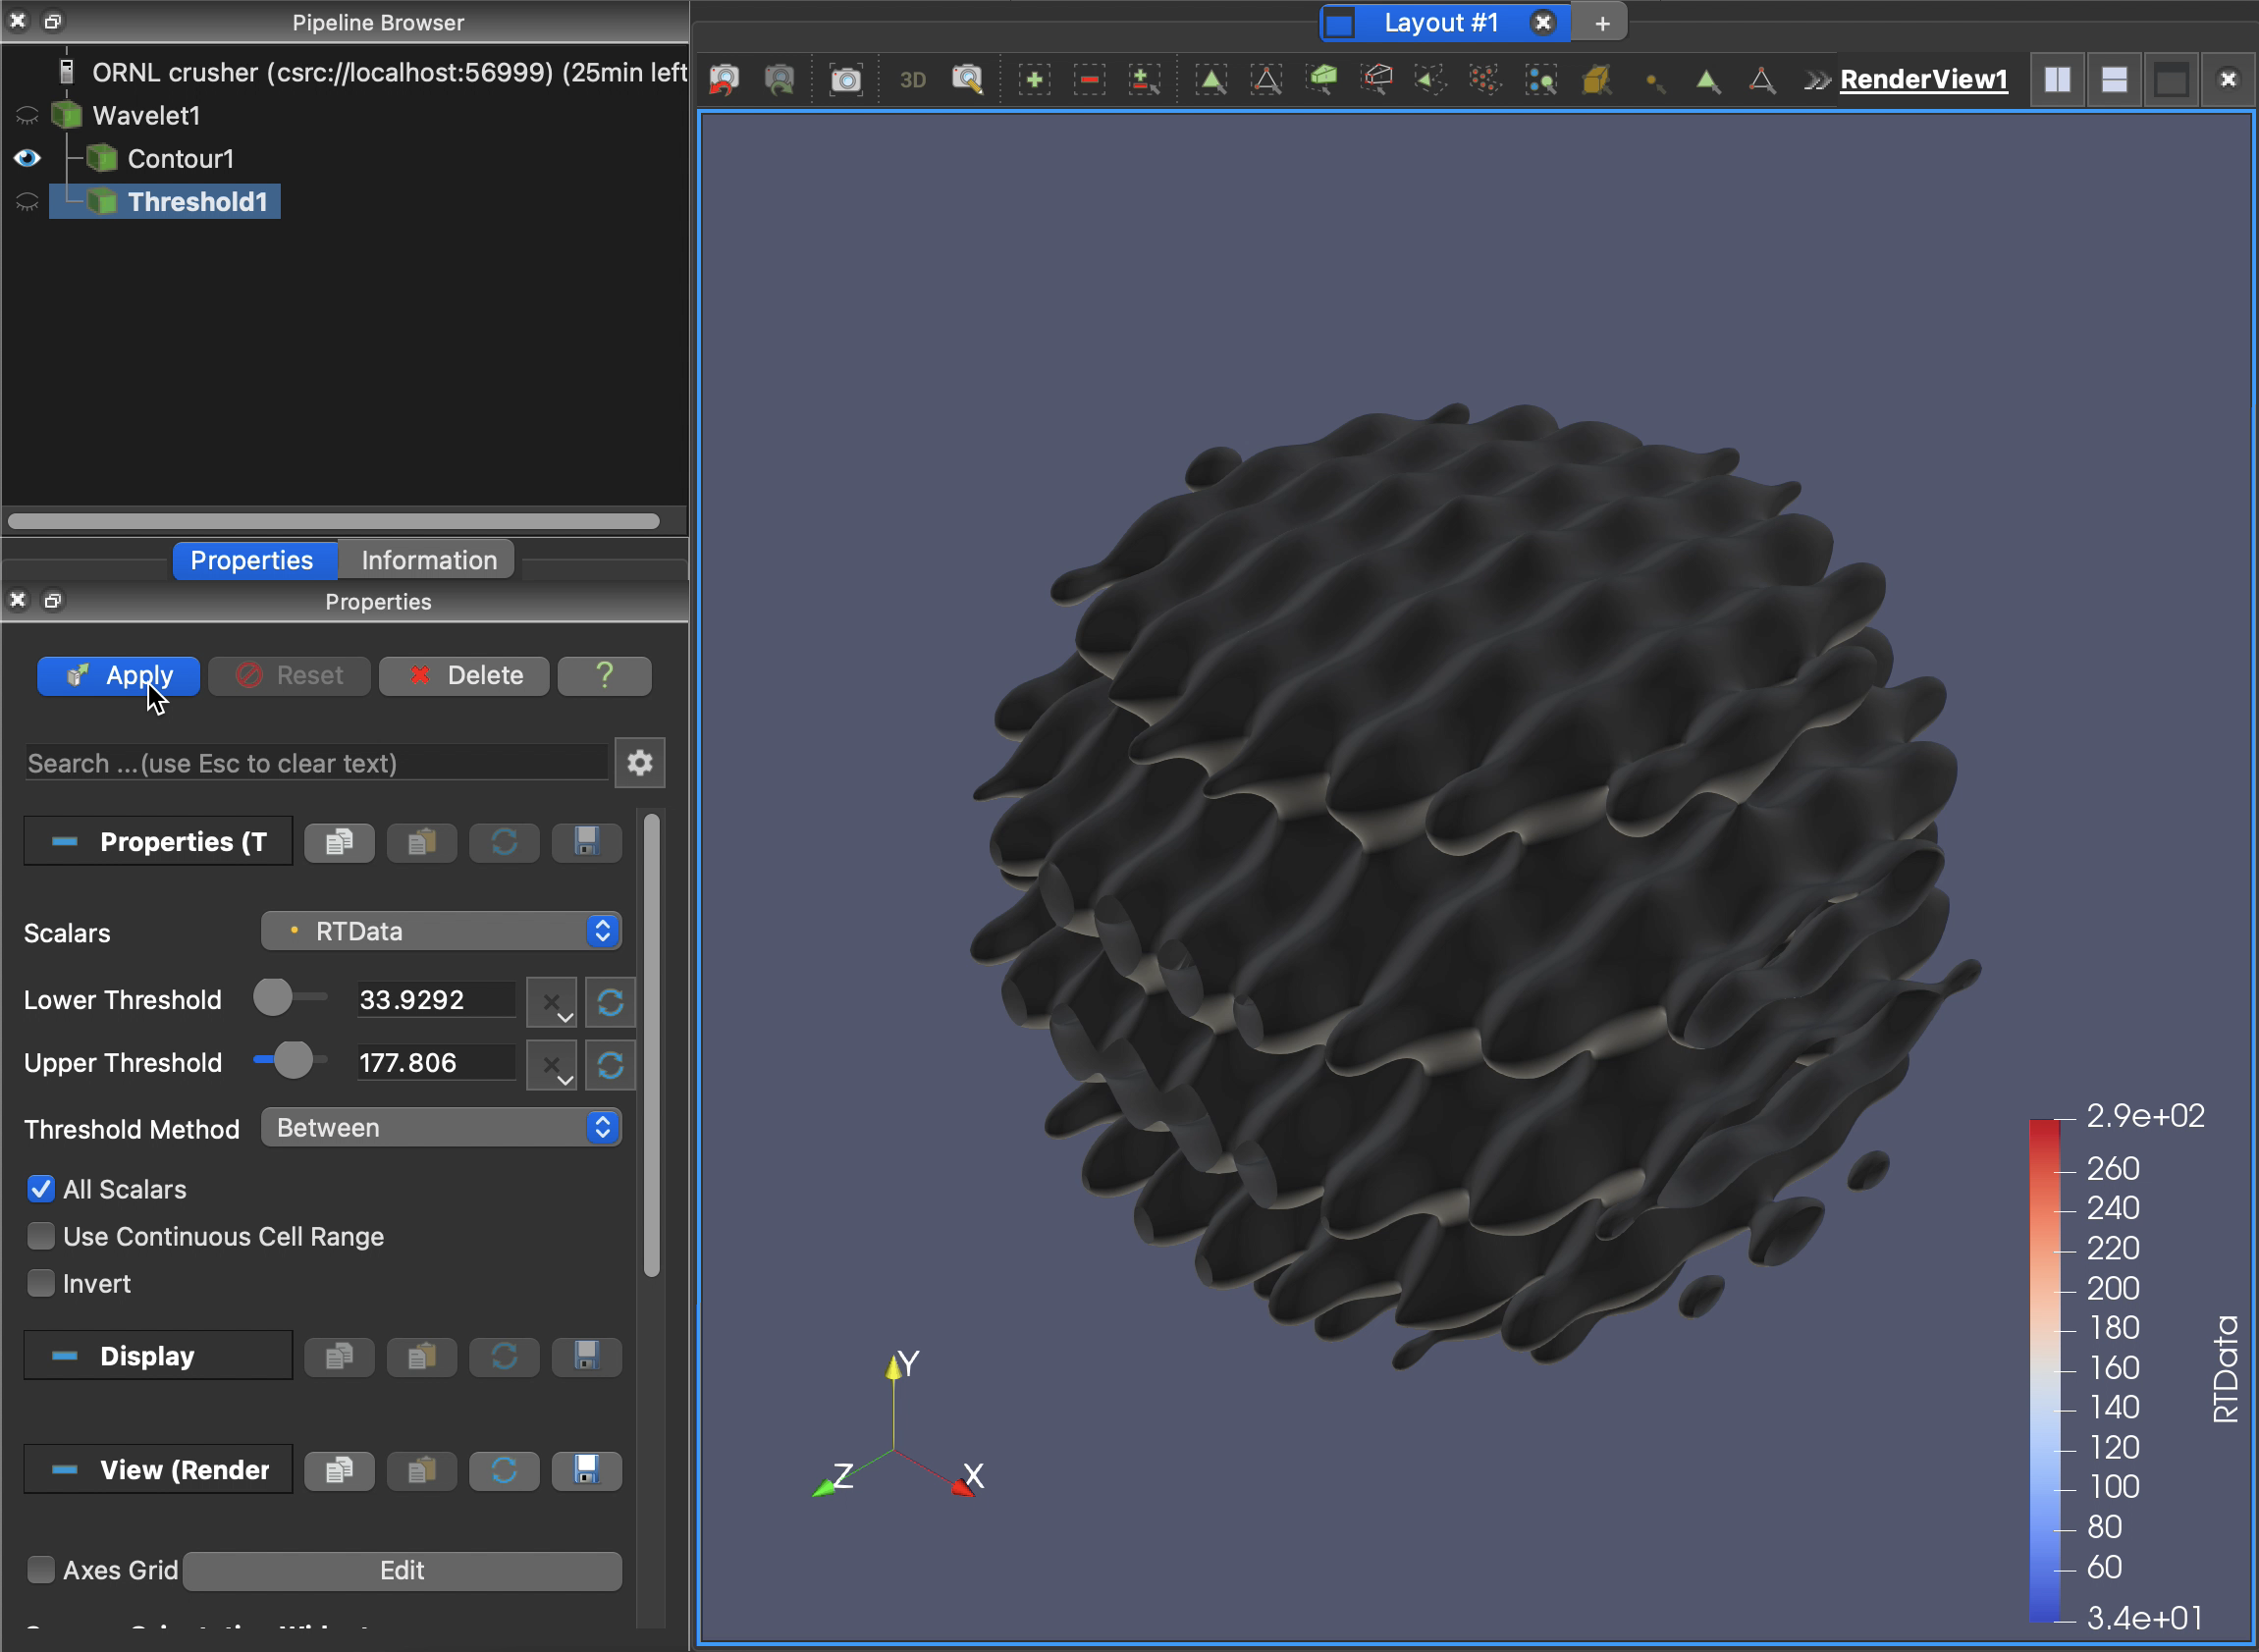
\includegraphics[width=\linewidth]{figures/paraview-crusher.png}
  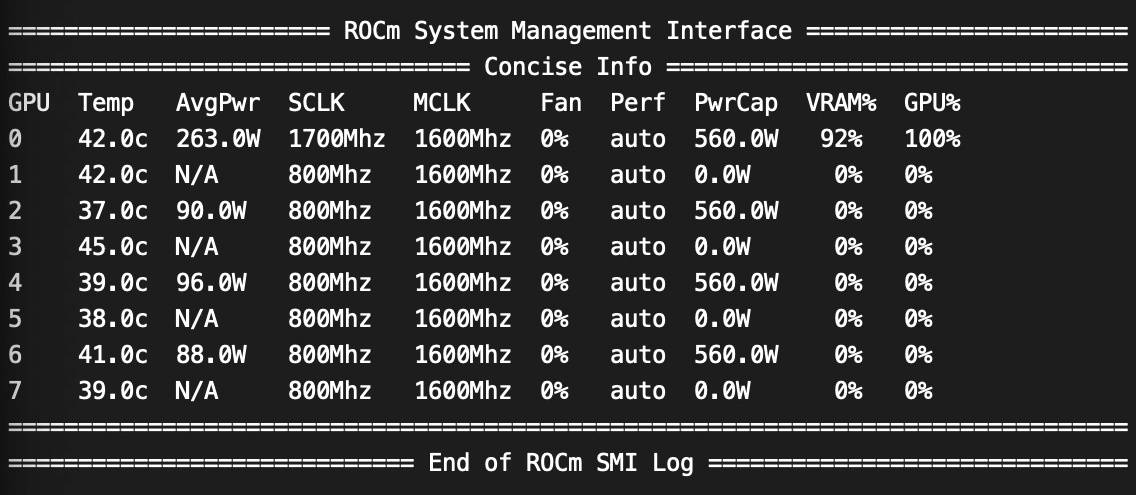
\includegraphics[width=\linewidth]{figures/threshold-vtkm-gpu-usage-crusher-small.png}
  \caption{
    ParaView with integrated \vtkm accelerated filters running on Crusher, an early access test bed for the Frontier system.
    \vtkm is using the Kokkos device adapter.
    The output of the \texttt{rocm-smi} command is being used to verify and monitor GPU usage by the filters.
    %\ken{I think it would be better to move this figure (or something like it) to the ParaView section.}
  }
  \label{fig:paraview-crusher}
\end{figure}

Figure~\ref{fig:paraview-crusher} shows an example of ParaView running with \vtkm accelerated filters on Crusher, which is an early access test bed for the Frontier system.
As described in the \nameref{sec:adopting-kokkos} section, \vtkm is using the Kokkos device adapter back end on this hardware.
The bottom of the image shows the output of the \texttt{rocm-smi} command, which is used to verify and monitor the GPU usage by the filters.

\begin{figure}[htb]
  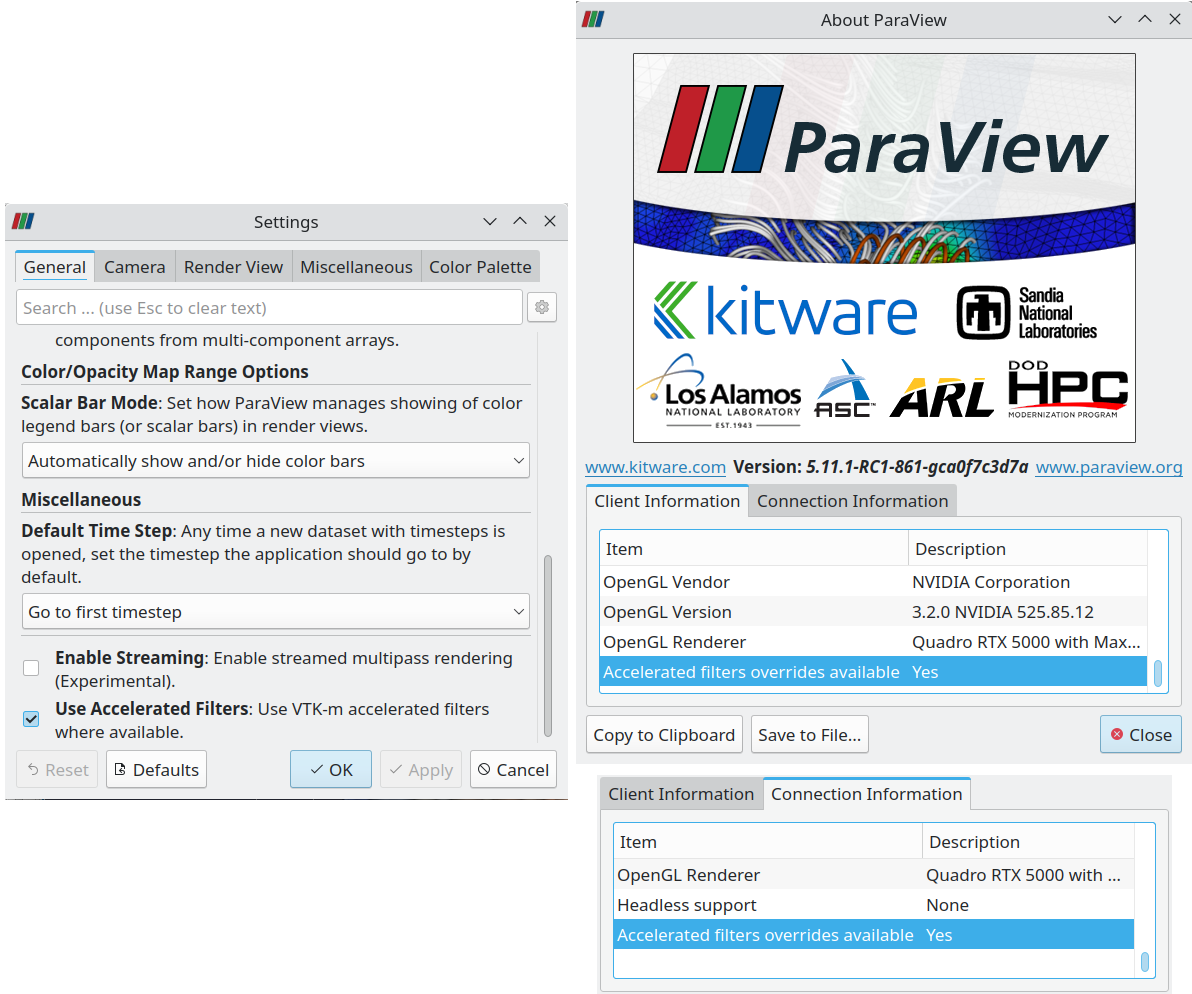
\includegraphics[width=\linewidth]{figures/pv-override-settings.png}
  \caption{
    Left: The \texttt{Use Accelerated Filters} ParaView setting can be used to activate or deactivate accelerated filter overrides at run time.
    This setting is shown regardless of whether or not ParaView was built with the override support.
    Right: The availability of the accelerated filter overrides on clients and servers can be found in the \texttt{About ParaView} dialog box.
  }
  \label{fig:paraview_settings}
\end{figure}

%\ken{This last paragraph might be more detail than needed.}
% The wrapper filter needs to be registered with the factory for the factory instantiation to work. This is done at the build configuration using the CMake function:
% \texttt{\_vtkm\_add\_override("vtkBaseFilter" "vtkmAcceleratedFilter")} Then, the accelerated filters need to be enabled using the CMake option \texttt{VTK\_ENABLE\_VTKM\_OVERRIDES}. They can also be turned on or off during run time through ParaView settings as shown in Figure~\ref{fig:paraview_settings}.
%\sujin{Ken, please review if the changes are satisfactory}
\vtkm accelerated filter overrides are available in recent releases of ParaView and can be enabled during building.
If enabled, the overrides can also be turned on or off at run time using the ParaView settings (Figure~\ref{fig:paraview_settings}).

\subsection{VisIt}

%\assign{Eric}
VisIt is a scientific visualization and analysis tool that operates on mesh-based field data.
Its functionality is grouped into four major categories: plots, operators, expressions, and queries.
All four of these capabilities are built on a filter infrastructure that operates on mesh-based fields.
Plots are somewhat special in that they consist of a rendering capability that may include some built-in filter operations.
To date, the \vtkm integration has consisted of modifying the filter infrastructure to use \vtkm filters when comparable \vtkm functionality exists.
%There has not yet been an effort to utilize \vtkm's rendering capabilities.


Previously, VisIt's filters used VTK filters and VTK datasets.
The filters were enhanced to support using both VTK and \vtkm.
When \vtkm is enabled in VisIt and the filter supports \vtkm, the filter will use \vtkm.
The internal dataset representation was also modified to support providing either a VTK dataset or a \vtkm dataset.
When the filter is set to use VTK, it will request the data as a VTK dataset or convert the dataset to a VTK dataset if it is stored as \vtkm.
Conversely, when the filter is set to use \vtkm, it will request the data as a \vtkm dataset and convert it if necessary.
It will use zero-copy conversions whenever possible.

\begin{figure}[htb]
  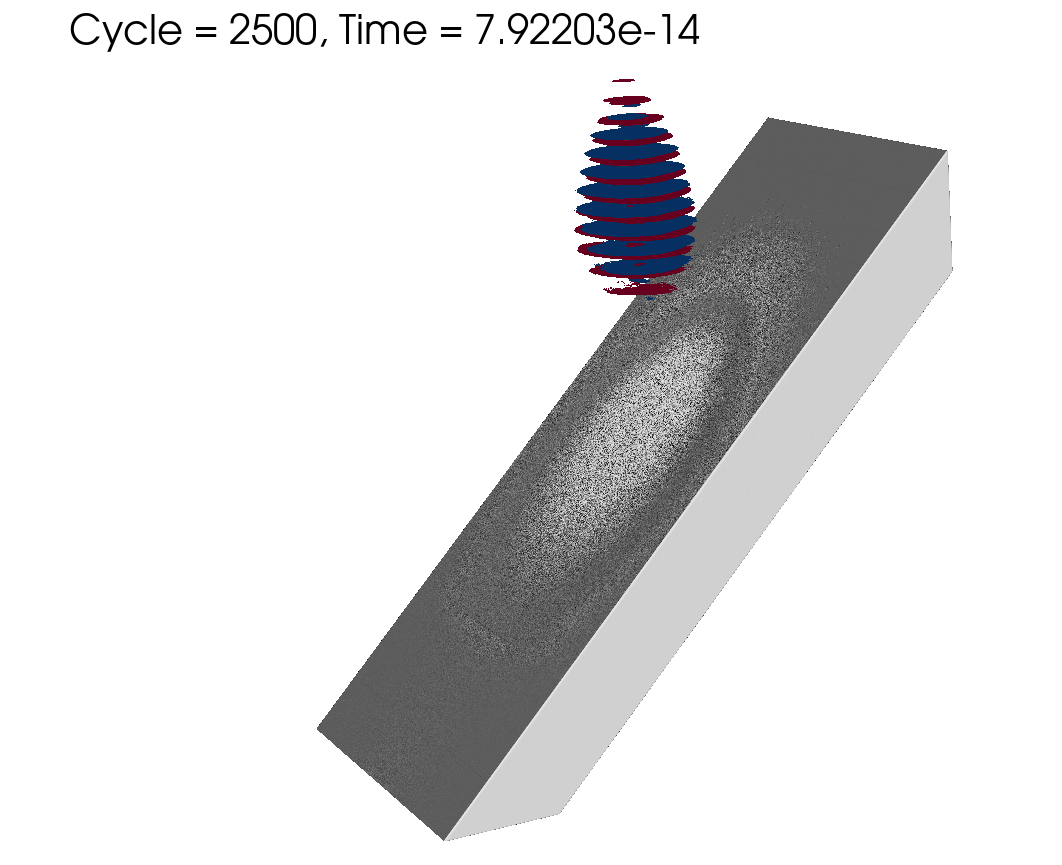
\includegraphics[width=\linewidth]{figures/visit_warpx_frontier.png}
  \caption{Visualization from a 70-billion cell WarpX simulation and Gordon Bell submission~\citep{FedeliHuebl2022} visualized with 2,048 GCDs on Frontier using VisIt.}
  \label{fig:visit_warpx_frontier}
\end{figure}

Figure~\ref{fig:visit_warpx_frontier} is an image generated by VisIt running on Frontier and using 2,048 GCDs across 256 nodes.
The surfaces were generated by using the \vtkm contour filter and were rendered in parallel by using Mesa 3D.
\vtkm is using the Kokkos back end for AMD GPUs.

\subsection{Ascent}

%\assign{Nicole}
Ascent is a lightweight, in-situ visualization and analysis library designed for running multiphysics simulations on HPC systems. As an in-situ library as opposed to a post-hoc visualization tool, Ascent shares execution resources with the simulation and can process the data as it is generated, thereby reducing I/O costs, although it must pause the simulation to do so. To minimize the encumbrance on the simulation and execution resources, Ascent's lightweight design ensures a smaller memory requirement. It is written using efficient distributed-memory and many-core libraries to guarantee performance and scalability on current and next-generation HPC platforms. Ascent has three main use cases: creating pictures, transforming data, and capturing data. Ascent is easy to use with only five API calls; supported in C, C++, Python, and Fortran; and provides an infrastructure to integrate custom analysis.
The data interface between simulation code and Ascent is managed through the Conduit API~\citep{Harrison2022}, which provides a simplified interface for passing data and describing structure.

Although optional, \vtkm is a dependency for Ascent because it is currently the only option for rendering low-order mesh data and provides filters for transforming and/or analyzing the simulation data (e.g.,
slice, histogram, contour).
Ascent also leverages \vtkm's zero-copy capabilities as well as its ability to pass device-pointers; these features allow the simulation data to remain on the device and be passed directly to Ascent and then on to \vtkm without being transferred to host memory.
\vtkm has been integrated into Ascent via a (previously external) library called VTK-h (VTK hybrid) that combines \vtkm's shared-memory, high-performance filters with MPI's efficient distributed-memory coordination.

\begin{figure}[b]
    \centering
    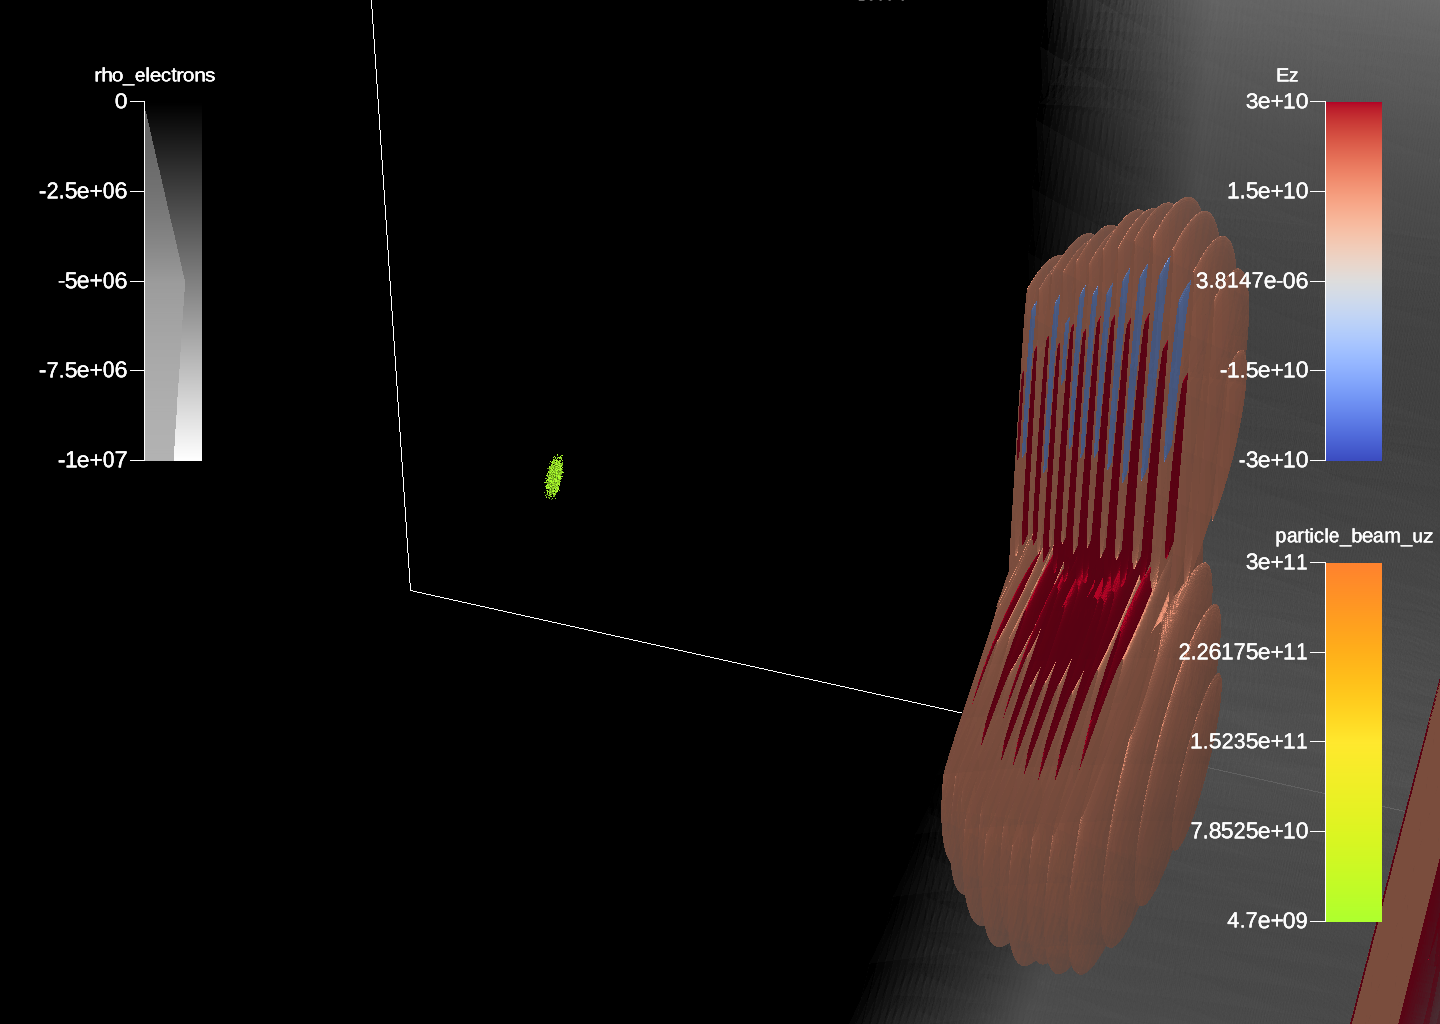
\includegraphics[width=\linewidth]{figures/ez_007050.png}
    \caption{WarpX in-situ visualization of a laser-wakefield accelerator on 4,416 GCDs across 552 nodes of Frontier using Ascent and \vtkm. The image depicts an early time step of the simulation at high resolution.}
    \label{fig:warpx_highres}
\end{figure}

\begin{figure}[t]
    \centering
    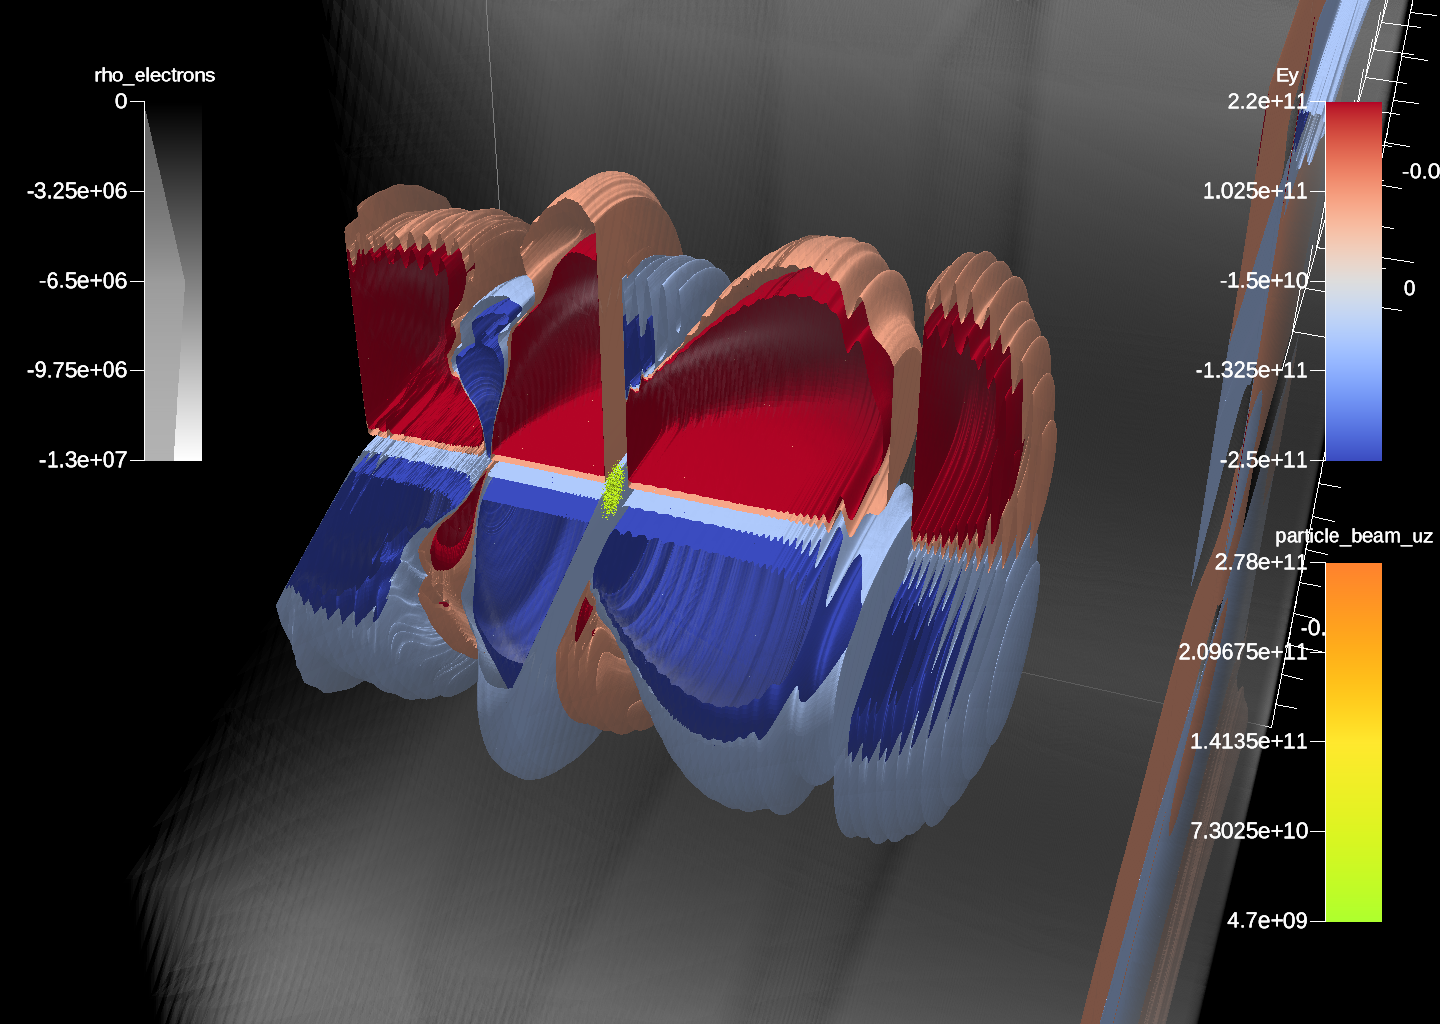
\includegraphics[width=\linewidth]{figures/ey_009300.png}
    \caption{WarpX in-situ visualization of a laser-wakefield accelerator on 552 GCDs across 69 nodes of Frontier using Ascent and \vtkm. The image depicts a later time step of the simulation at low resolution.}
    \label{fig:warpx_lowres}
\end{figure}

Figures~\ref{fig:warpx_highres} and~\ref{fig:warpx_lowres} show in-situ renderings of the WarpX simulation (see the \nameref{sec:warpx} section later in this paper) generated by Ascent and executed on the OLCF's exascale supercomputer, Frontier.
The simulation was executed at two resolutions: 578.8 million cells across 552 GCDs on 69 nodes and 4.63 billion cells across 4,416 GCDs on 552 nodes.
Ascent used \vtkm filters to upscale the data along multiple axes, generate isosurfaces, and clip several fields before using \vtkm's raytracer and volume renderer to generate the final images.
To guarantee performance, \vtkm uses the Kokkos back end for AMD GPUs. 

%\begin{figure}[htb]
%  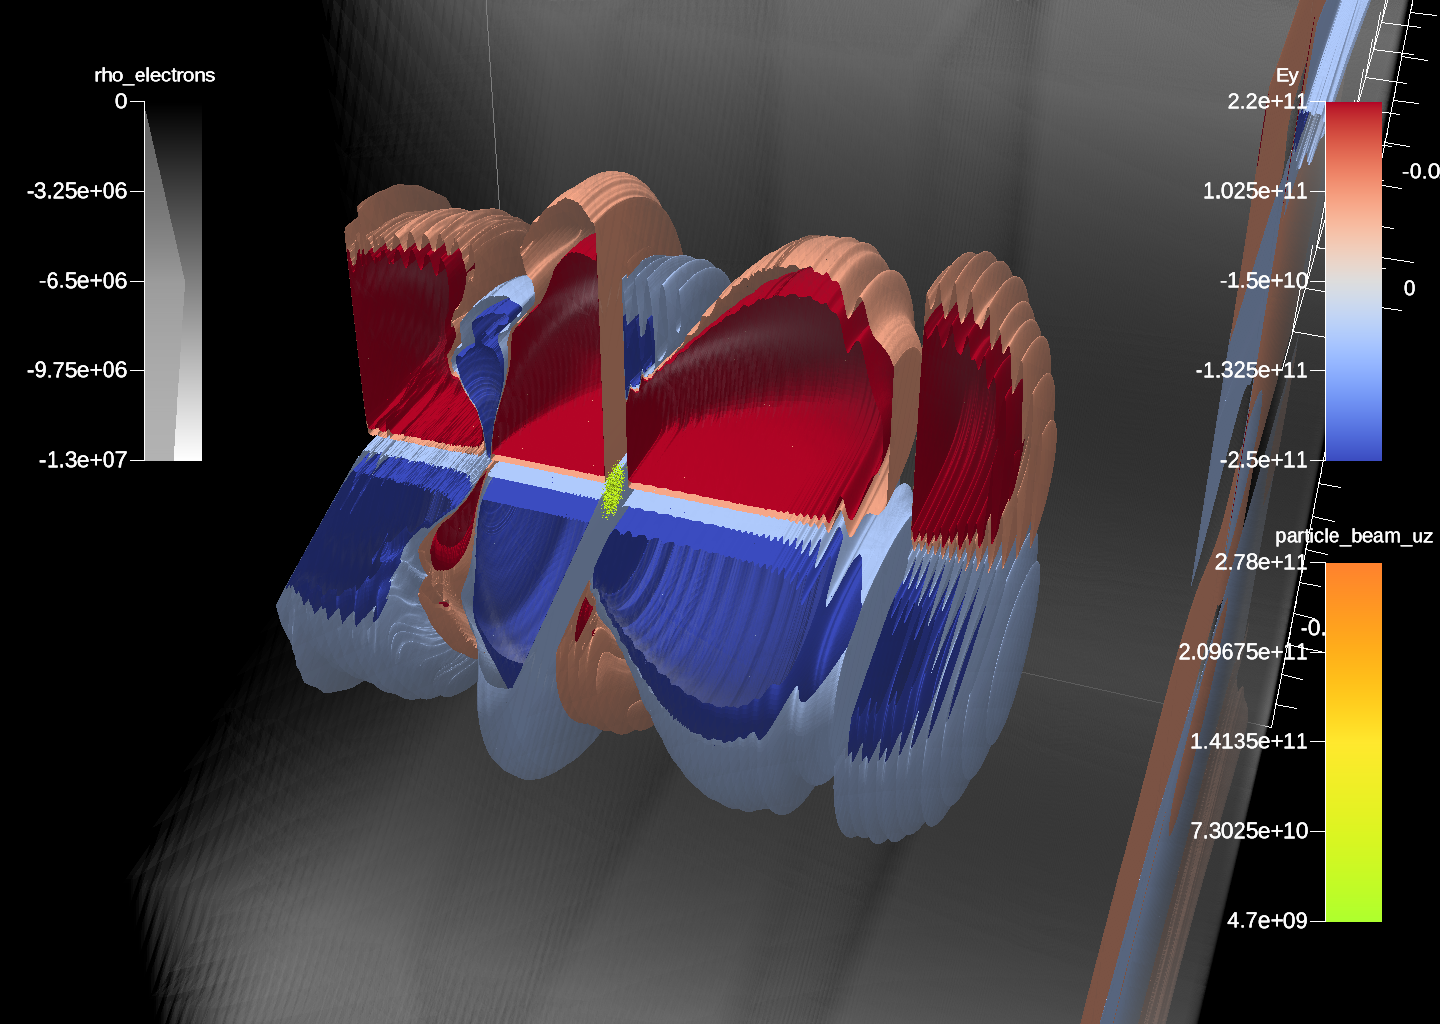
\includegraphics[width=\linewidth]{figures/warpx_stages_lwfa.png}
%  \caption{WarpX in situ visualization of a laser-wakefield accelerator on 552 nodes containing 4,416 GPUs on Frontier using Ascent and \vtkm.
%  The inset shows an early simulation time step at high resolution.}
%  \label{fig:warpx_lwfa}
%\end{figure}

\subsection{Alternative Delivery Mechanisms}

%\assign{Tushar}

Integrating a new feature that was implemented with \vtkm filters into visualization software such as ParaView or VisIt can be a lengthy process.
For example, making a \vtkm filter available in ParaView requires multiple steps, including implementing a VTK filter that wraps the \vtkm filter, completing the arduous process of contributing the change to the VTK project, and then repeating similar steps in ParaView itself.
Such time-consuming software integration can hinder the availability of \vtkm filters inside visualization tools and limit the opportunities for \vtkm filters to increase the pace of scientific discovery.

Our ultimate goal is to make \vtkm filters practical for real use and to put tools in the hands of end users in a timely manner.
An alternative approach to a full integration through the visualization software stack is to provide this functionality through a plug-in that is supported by tools such as ParaView and VisIt.
For the plug-in approach, the \vtkm filter is still wrapped inside a VTK filter, but the time needed for the software integration and testing in VTK and ParaView can be bypassed.

Figure~\ref{fig:uncertainty-plugin} illustrates the \vtkm isosurface uncertainty filter~\citep{Wang2023, Athawale21} made available in ParaView via the plug-in method. The isosurface uncertainty filter is one of the major successes of the \vtkm library because it is the first production-level uncertainty visualization filter deployed for efficient large-data analysis. Using the plug-in method depicted in Figure~\ref{fig:uncertainty-plugin}, \vtkm filters can be easily combined with existing filters in ParaView for improved data comprehension.

\begin{figure}[htb]
  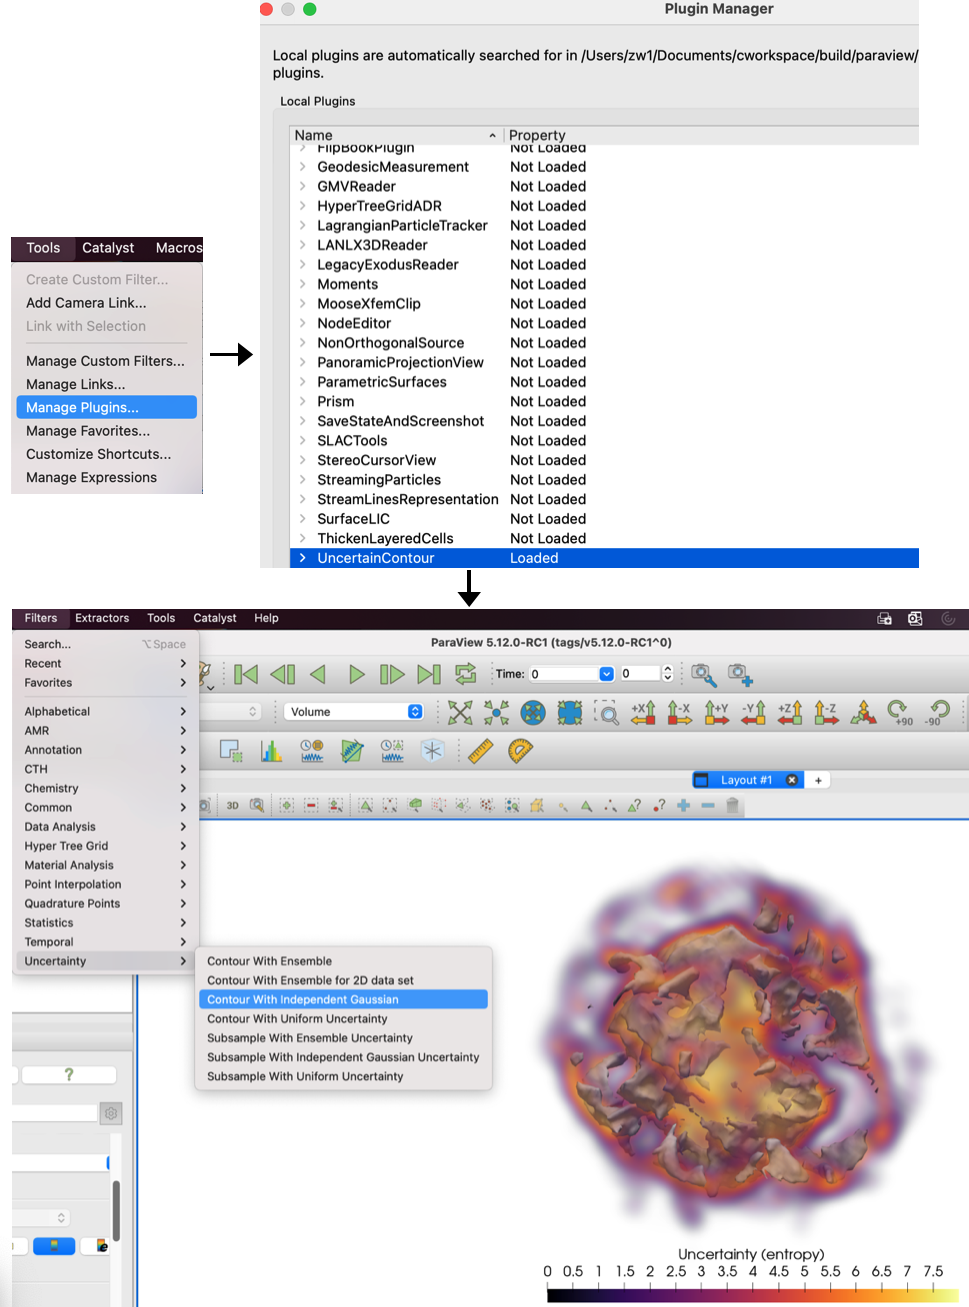
\includegraphics[width=\linewidth]{figures/isosurfaceUncertaintyPlugin.png}
  \caption{Integration of the \vtkm isosurface uncertainty filter in ParaView using the plug-in approach for visualization of large-scale supernova simulations~\citep{Sandoval2021}.}
  \label{fig:uncertainty-plugin}
\end{figure}



%% \ken{
%%   Talk about how you can deliver new functionality to these tools outside of the pipeline of implement in \vtkm $\rightarrow$ VTK $\rightarrow$ Tool.
%%   Use uncertainty plugin as an example of doing this.
%% }
